\section{Чувствительность к структуре Земли}
%\subsection{Потоки как функция зенитного угла}
%\subsection{Зависимость от энергии}
\subsection{Спектроскопия ядра Земли с нейтрино}
При прохождении нейтрино сквозь Землю мы должны учитывать, что нейтрино в толще земли может взаимодействовать посредством заряженного и нейтрального токов. В качестве примера рассмотрим следующий модельный поток нейтрино на поверхности Земли: 
\begin{equation}
    F_{\nu}^{0}(E) = K\left(\frac{E_0}{E}\right)^{\gamma+1} (1+E_0/E)^{-\alpha}\phi\left(\frac{E}{E_{cut}}\right),
\end{equation}
где $\phi_{cut}(t)$ - некоторая функция, предназначенная для резкого обрезания потоков при энергиях выше некоторого порога. В качестве такой функции возьмем следующую функцию:
\begin{equation}
    \phi(t) = (1+\tan(\pi t/2))^{-1}
\end{equation}
В дальнейшем будем считать, что $\gamma = 1$ и $\alpha = 0.5$.
В качестве точки взаимодействия нейтрино возьмем точку на глубине 1 км от поверхности Земли. Эволюцию потоков нейтрино при прохождении сквозь Землю можно увидеть на рис. (\ref{EF1}). Здесь $\theta_d$ - угол прилета нейтрино относительно детектора (схематическое расположение углов можно увидеть на рис. (\ref{EF1}) справа), $\Phi_{CC}(\theta_d, E)$  - потоки нейтрино в детекторе, если бы мы учитывали изменение только за счет заряженного тока, $\Phi_{CC+NC}(\theta_d, E)$  - потоки нейтрино в детекторе, если бы мы учитывали изменение за счет заряженного и нейтрального токов. Можно видеть, что при энергиях нейтрино выше 1 ПэВ нейтральный ток начинает оказывать большой эффект при распространении нейтрино сквозь Землю. Особенно эффект становится ощутим, если траектория нейтрино проходит через ядро Земли. Данная картинка подсказывает нам эксперимент по спектрографии Земли. Если взять пучок нейтрино высоких энергий (1 ТэВ) и пустить его сквозь Землю по диаметру, поставив два детектора с противоположных сторон, мы сможем измерять потоки нейтрино до и после их прохождения через Землю. Так как при распространении нейтрино практически не изменяет своего направления, можно учесть эффект поглощения нейтрино за счет заряженного тока. Таким образом, превышение потоков нейтрино во втором детекторе от ожидаемых потоков (изменившихся только за счет поглощения) позволит оценить плотность ядра Земли (т. к. основной эффект увеличения потоков дает именно ядро).   
\begin{figure}[!h]
\centering
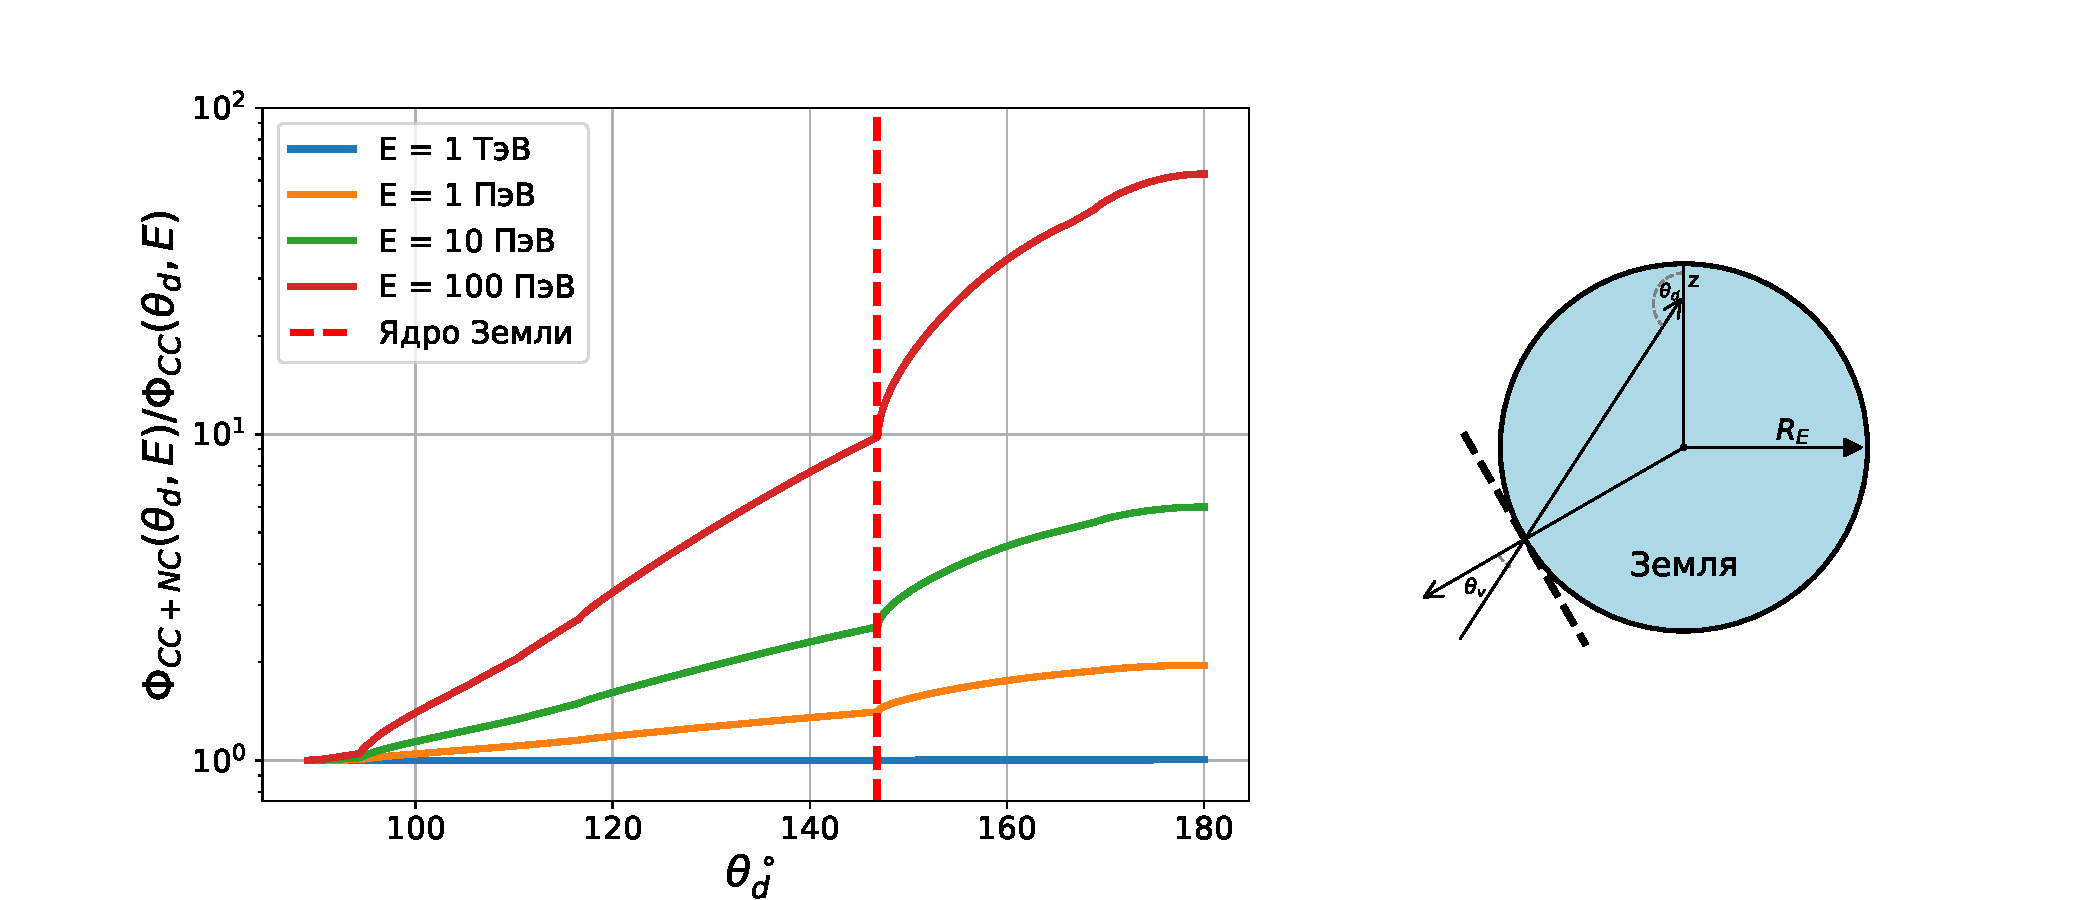
\includegraphics[width=1.1\linewidth]{"images/NuProp/rhh12zf_flux_index_CT18ZNNLO.pdf"}
\caption{Вклад взаимодействий нейтрино за счет нейтрального тока в общий поток в точке наблюдения потока в зависимости от угла прилета нейтрино отностиельно детектора для разных значений энергии нейтрино. Здесь $z$ - глубина, на которой находится детектор, $\theta_d$ - угол прилета нейтрино, относительно детектора, $\theta_n$ - угол прилета нейтрино, относительно нормали к Земле, $R_E$ - Радиус Земли.}
\label{EF1}
\end{figure}
При распространении нейтрино от одной точки в другую через толщу вещества учитывается как обычный фактор затухания нейтрино, так и фактор, связанный с регенерацией потока (учет реакций, когда конечным лептоном является также нейтрино). В соответствии с процедурой, описанной ранее, для потоков мюонных нейтрино можно построить соответствующую экспоненциальную поправку к затуханию. Полную же картину распространения нейтрино можно увидеть на рис. (\ref{EF2}).
\subsection{Поглощение нейтрино в среде }
 Полную картину распространения нейтрино в зависимости от энергии нейтрино и зенитного угла относительно детектора  можно увидеть на рис. (\ref{EF2}). Здесь учтено поглощение потока, которое дается экспоненциальной поправкой, и регенерация потока, рассчитанная с помощью процедуры Z-фактора.
 \begin{figure}[!h]
\centering
\includegraphics[width=1.1\linewidth]{"images/NuProp/rzf_2dxsTUJU19_nlo_2_1.png"}
\caption{Вероятность прохождения нейтрино сквозь Землю в зависимости от энергии и зенитного угла, измеряющегося относительно детектора.}
\label{EF2}
\end{figure}
\subsection{Поглощение за счет нейтрального и заряженного токов}
В конце зададимся вопросом, как изменяется показатель потока при прохождении нейтрино сквозь Землю за счёт разных взаимодействий. Предположим, что начальный и конечный потоки имеют форму 
\begin{equation}
    F_{in/fin}(E) = \Phi_0 E^{-\gamma_{in/fin}(E)}.
\end{equation}
На рис. (\ref{EF3}) можно видеть, что показатель потока начинает сильно изменяться при энергиях выше 10 ТэВ. Таким образом, для нейтрино высоких энергий, проходящих сквозь Землю, спектр будет сильно изменяться, поэтому количество событий для таких нейтрино будет сильно меньше ожидаемых. Нейтрино же, летящие сверху, не подвергнутся такому подавлению потока.    
\begin{figure}[!h]
\centering
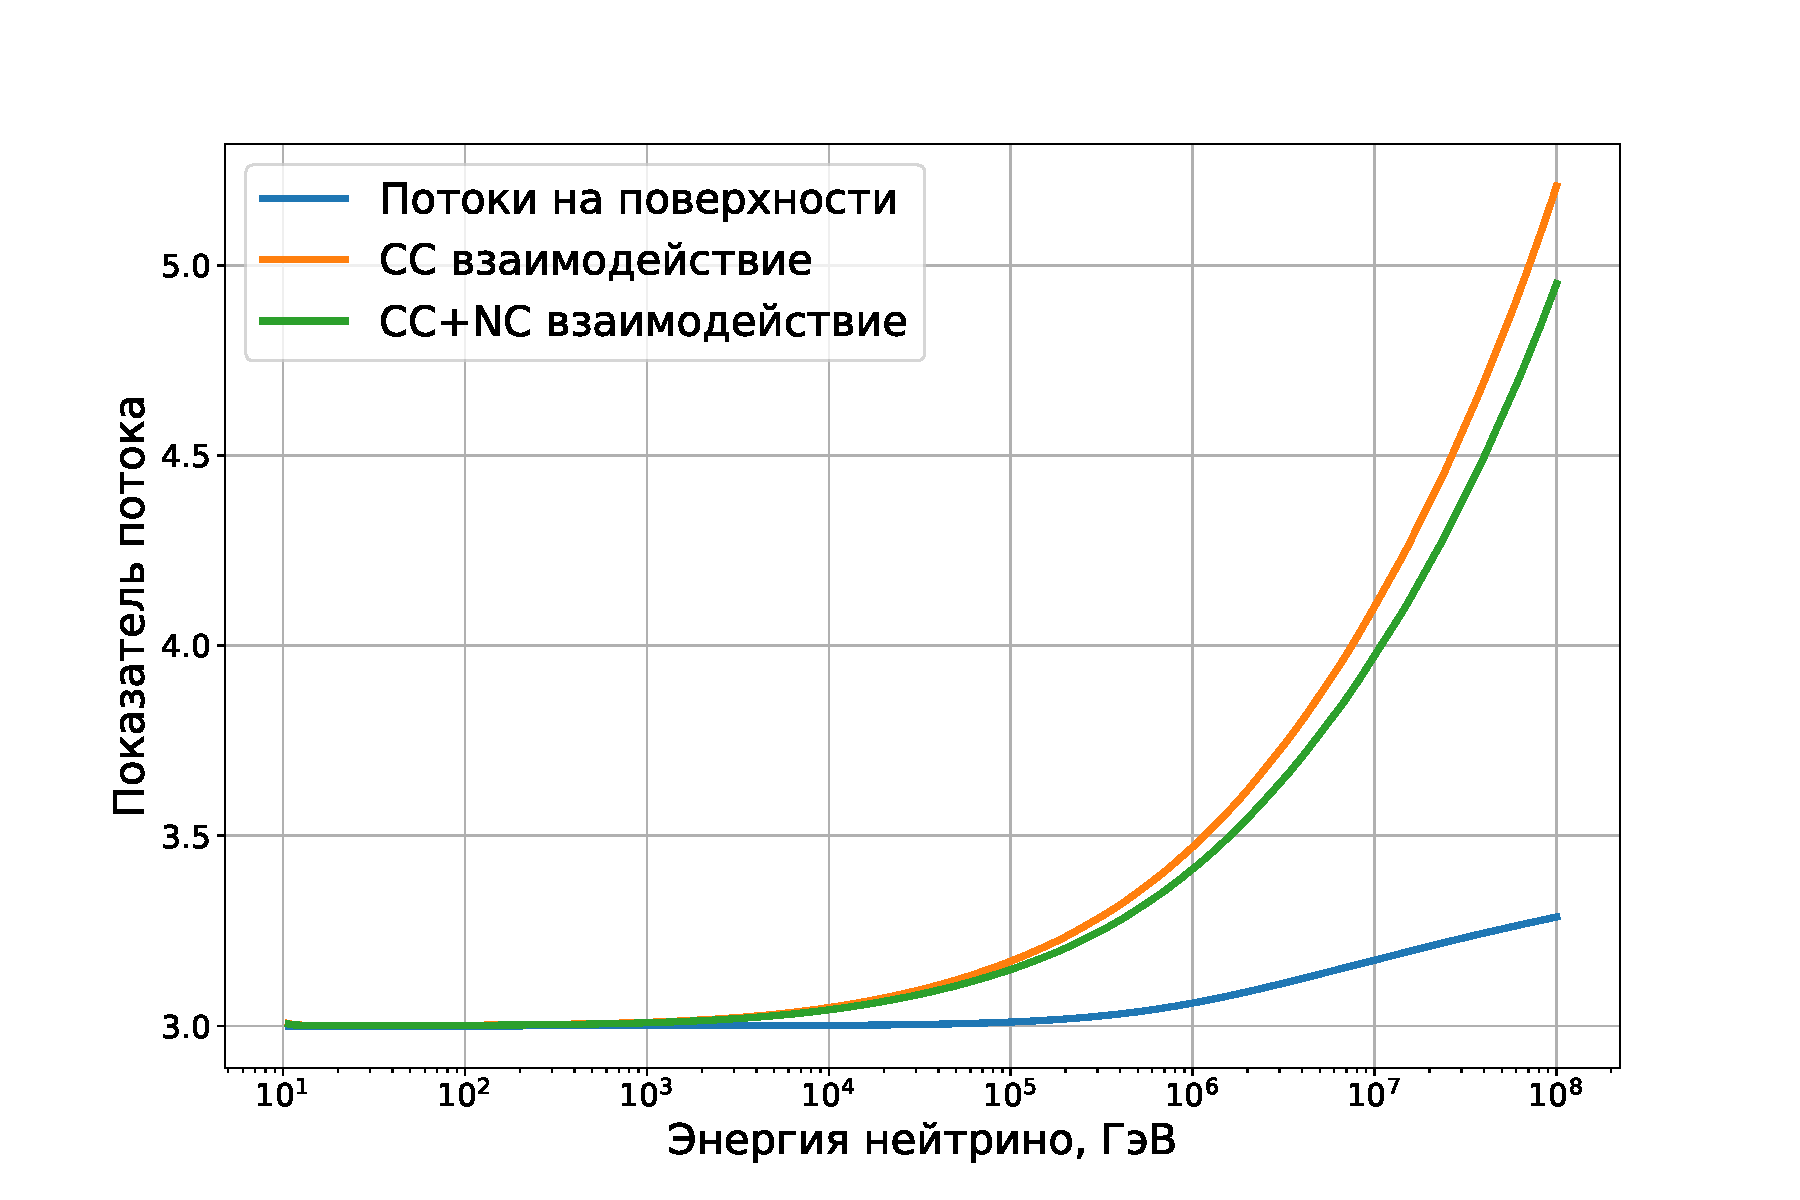
\includegraphics[width=1.1\linewidth]{"images/NuProp/rzf_flux_index_CT18ZNNLO.pdf"}
\caption{Изменение показателя потока нейтрино для пучка, проходящего сквозь Землю в зависимости от энергии при учете разных типов взаимодействия.}
\label{EF3}
\end{figure}
\subsection{Томография Земли с помощью нейтрино}
Рассмотрим возможность уточнить плотность Земли с помощью нейтрино. На данный момент вся информация о плотности Земли получена косвенным образом из сейсмологических данных~\cite{PREM}. Однако, можно получать также информацию о плотности с помощью распространения нейтрино в Земле. Одни анализы основаны на осцилляциях нейтрино низких энергий в веществе. В случае же высоких энергий длина осцилляции намного больше радиуса Земли, поэтому осцилляциями можно пренебречь. Однако есть другой способ, основанный на том, что при прохождении нейтрино сквозь Землю происходят два конкурирующих процесса. С одной стороны, потоки нейтрино убывают за счет поглощения нейтрино в среде. С другой стороны, потоки перераспределяются за счет взаимодействия по нейтральному току (обсуждавшийся выше эффект регенерации). В зависимости от длины пути и от плотности вещества вдоль этого пути, мы будем получать разные числа событий в детекторе.


В данной работе мы проведем анализ, предположив, что у нас есть две гипотезы: $H_0$ и $H_1$. Гипотеза $H_0$ будет утверждением о том, что модель плотности PREM верна. В качестве альтернативной гипотезы будем рассматривать простейшие отклонения от данной модели.   
Рассмотрим три альтернативные модели: модель с усредненным ядром, модель с линейным ядром и модель с усредненными мантией и ядром. Анализ будем проводим с помощью статистики $\chi^2$. Найдем полные числа событий нейтринном телескопе объемом $1\text{ км}^3$ за один год для каждой из гипотез и на основании статистики примем либо отклоним гипотезу $H_0$. $\chi^2$ будем рассчитывать по формуле 
\begin{equation}
    \Delta\chi^2 = 2\sum\limits_{ij}(N_{ij}^{(0)} - N_{ij}^{(1)}+N_{ij}^{(1)}\ln(N_{ij}^{(1)}/N_{ij}^{(0)})),
\end{equation}
где $N^{k}_{ij}$ - количество нейтринных событий в определенном диапазоне по углам и энергии, соответствующих $k$-й гипотезе. 
\begin{enumerate}
    \item \textbf{Усредненное ядро и мантия.} В качестве альтернативной гипотезы возьмем модель плотности, равной $5.51\text{ г/см}^3$ в области внутреннего ядра, внешнего ядра и мантии (до 5600 км).В остальной же области модель будет совпадать с моделью PREM. Для данной пары ($H_0$,$H_1$) получилось $\Delta\chi^2 = 12.2$, что соответствует статистической значимости на уровне $3.4936\sigma$.   
    \begin{figure}[!h]
    \centering
    \includegraphics[width=1.1\linewidth]{"images/NuProp/chi2_rzf_2dxsCT18ZNNLO_PREM_vs_PREM_man_and_ker.png"}
    \caption{Распределение $\Delta\chi^2$, полученное на основе сравнения чисел нейтринных событий в предположении двух гипотез, где в качестве альтернативной гипотезы взята гипотеза усредненного ядра и мантии}
    \label{NuTom1}
    \end{figure}
    \item \textbf{Усредненное ядро.} В качестве альтернативной гипотезы возьмем модель плотности, равной $11.87\text{ г/см}^3$ в области внутреннего ядра и внешнего ядра. В остальной же области модель будет совпадать с моделью PREM. Для данной пары ($H_0$,$H_1$) получилось $\Delta\chi^2 = 0.15$, что соответствует статистической значимости на уровне $0.3873\sigma$. Если проводить наблюдения в течение 25 лет или же анализировать данные, полученные с помощью очень больших нейтринных телескопов (объемом $30 \text{ км}^3$, например), то результат станет статистически значимым на уровне $2\sigma$.   
    \begin{figure}[!h]
    \centering
    \includegraphics[width=1.1\linewidth]{"images/NuProp/chi2_rzf_2dxsCT18ZNNLO_PREM_vs_PREM_av_ext_ker.png"}
    \caption{Распределение $\Delta\chi^2$, полученное на основе сравнения чисел нейтринных событий в предположении двух гипотез, где в качестве альтернативной гипотезы взята гипотеза усредненного ядра}
    \label{NuTom2}
    \end{figure}
    \item \textbf{Линейное ядро.} Теперь в качестве альтернативной гипотезы возьмем модель плотности,  где плотность аппроксимируется линейной функцией в области внутреннего ядра и внешнего ядра. В остальной же области модель будет совпадать с моделью PREM. Для данной пары ($H_0$,$H_1$) получилось $\Delta\chi^2 = 0.76$, что соответствует статистической значимости на уровне $0.8718\sigma$. Если проводить наблюдения в течение 10 лет, то результат станет статистически значимым на уровне $2.757\sigma$. 
    \begin{figure}[!h]
    \centering
    \includegraphics[width=1.1\linewidth]{"images/NuProp/chi2_rzf_2dxsCT18ZNNLO_PREM_vs_PREM_lin_ker.png"}
    \caption{Распределение $\Delta\chi^2$, полученное на основе сравнения чисел нейтринных событий в предположении двух гипотез, где в качестве альтернативной гипотезы взята гипотеза линейного ядра}
    \label{NuTom3}
    \end{figure}
\end{enumerate}
На основе распределений статистики $\Delta\chi^2$ (рис.~\ref{NuTom1} - рис.~\ref{NuTom3}) можно видеть, что диапазон энергии, особенно чувствительный для нейтринной томографии  - $10^2 \text{ГэВ}-10^6 \text{ГэВ}$, причем пик приходится на $10^4 \text{ ГэВ}$. В этой области среда становится непрозрачной для нейтрино и, в свою очередь, потоки еще не слишком маленькие, как при больших энергиях. Максимум же по углу зависит от того, какую альтернативную модель плотности мы рассматриваем (при изменении плотности в слое мантии, максимум по углам будет смещаться влево к меньшим углам). 
\subsection{Кинетические уравнения}
Рассмотрим уравнение переноса нейтрино, учитывая поглощение нейтрино и взаимодействие нейтрино в веществе.
\begin{equation}
    \frac{\partial F(E, x)}{\partial x} = -\sigma_{tot}(E)F(E, x) + \int\limits_{0}^1\frac{dy}{1-y}\frac{d\sigma_{tot}}{dy}(E_y, y)F(E_y, x), 
\end{equation}
где $E_y = E/(1-y)$ - энергия нейтрино до возможного рассеяния. Перепишем его в виде системы уравнений:
\begin{equation}
    \begin{cases}
         \frac{\partial F(E, x)}{\partial x} = -\sigma_{tot}(E)F(E, x) + Z(E, x)F(E, x),\\
          Z(E, x) = \int\limits_{0}^1\frac{dy}{1-y}\frac{d\sigma_{tot}}{dy}(E_y, y)F(E_y, x).
    \end{cases}
\end{equation}
Перепишем первое уравнение в интегральном виде:
\begin{equation}
    \begin{cases}
          F(E, x) = F_0(E)\exp{(-\sigma_{tot}(E)x + \int\limits_{0}^1dx_1Z(E, x_1)}),\\
          Z(E, x) = \int\limits_{0}^1\frac{dy}{1-y}\frac{d\sigma_{tot}}{dy}(E_y, y)F(E_y, x).
    \end{cases}
\end{equation}
\begin{equation}
    \begin{cases}
          F(E, x) = F_0(E)\exp{(-\sigma_{tot}(E)x + \int\limits_{0}^1dx_1Z(E, x_1)}),\\
          Z(E, x) = \int\limits_{0}^1\frac{dy}{1-y}\frac{d\sigma_{tot}}{dy}(E_y, y)F(E_y, x).
    \end{cases}
\end{equation}
Таким образом, мы получаем следующее интегральное уравнение: 
\begin{equation}
          F(E, x) = F_0(E)\exp{\left(-\sigma_{tot}(E)x + \int\limits_{0}^1dx_1 \int\limits_{0}^1\frac{dy}{1-y}\frac{d\sigma_{tot}}{dy}(E_y, y)\frac{F(E_y, x)}{F(E,x)}\right)}.
\end{equation}
Решаем его итерациями: 
\begin{equation}
          F^{(n+1)}(E, x) = F_0(E)\exp{\left(-\sigma_{tot}(E)x + \int\limits_{0}^1dx_1 \int\limits_{0}^1\frac{dy}{1-y}\frac{d\sigma_{tot}}{dy}(E_y, y)\frac{F^{(n)}(E_y, x)}{F^{(n)}(E,x)}\right)}.
\end{equation}
В первом приближении имеем: 
\begin{equation}
          F^{(1)}(E, x) = F_0(E)\exp{\left(-x\left[\sigma_{tot}(E) -\int\limits_{0}^1dy\frac{d\sigma_{tot}}{dy}(E_y, y)\eta(E, y)\right]\right)},
\end{equation}
где 
\begin{equation}
    \eta(E,y) = \frac{F_0(E_y)}{(1-y)F_0(E)}.
\end{equation}
